
\subsection{State  of  the Art}
    

\begin{figure}[t]
 %
 \centering
 %
 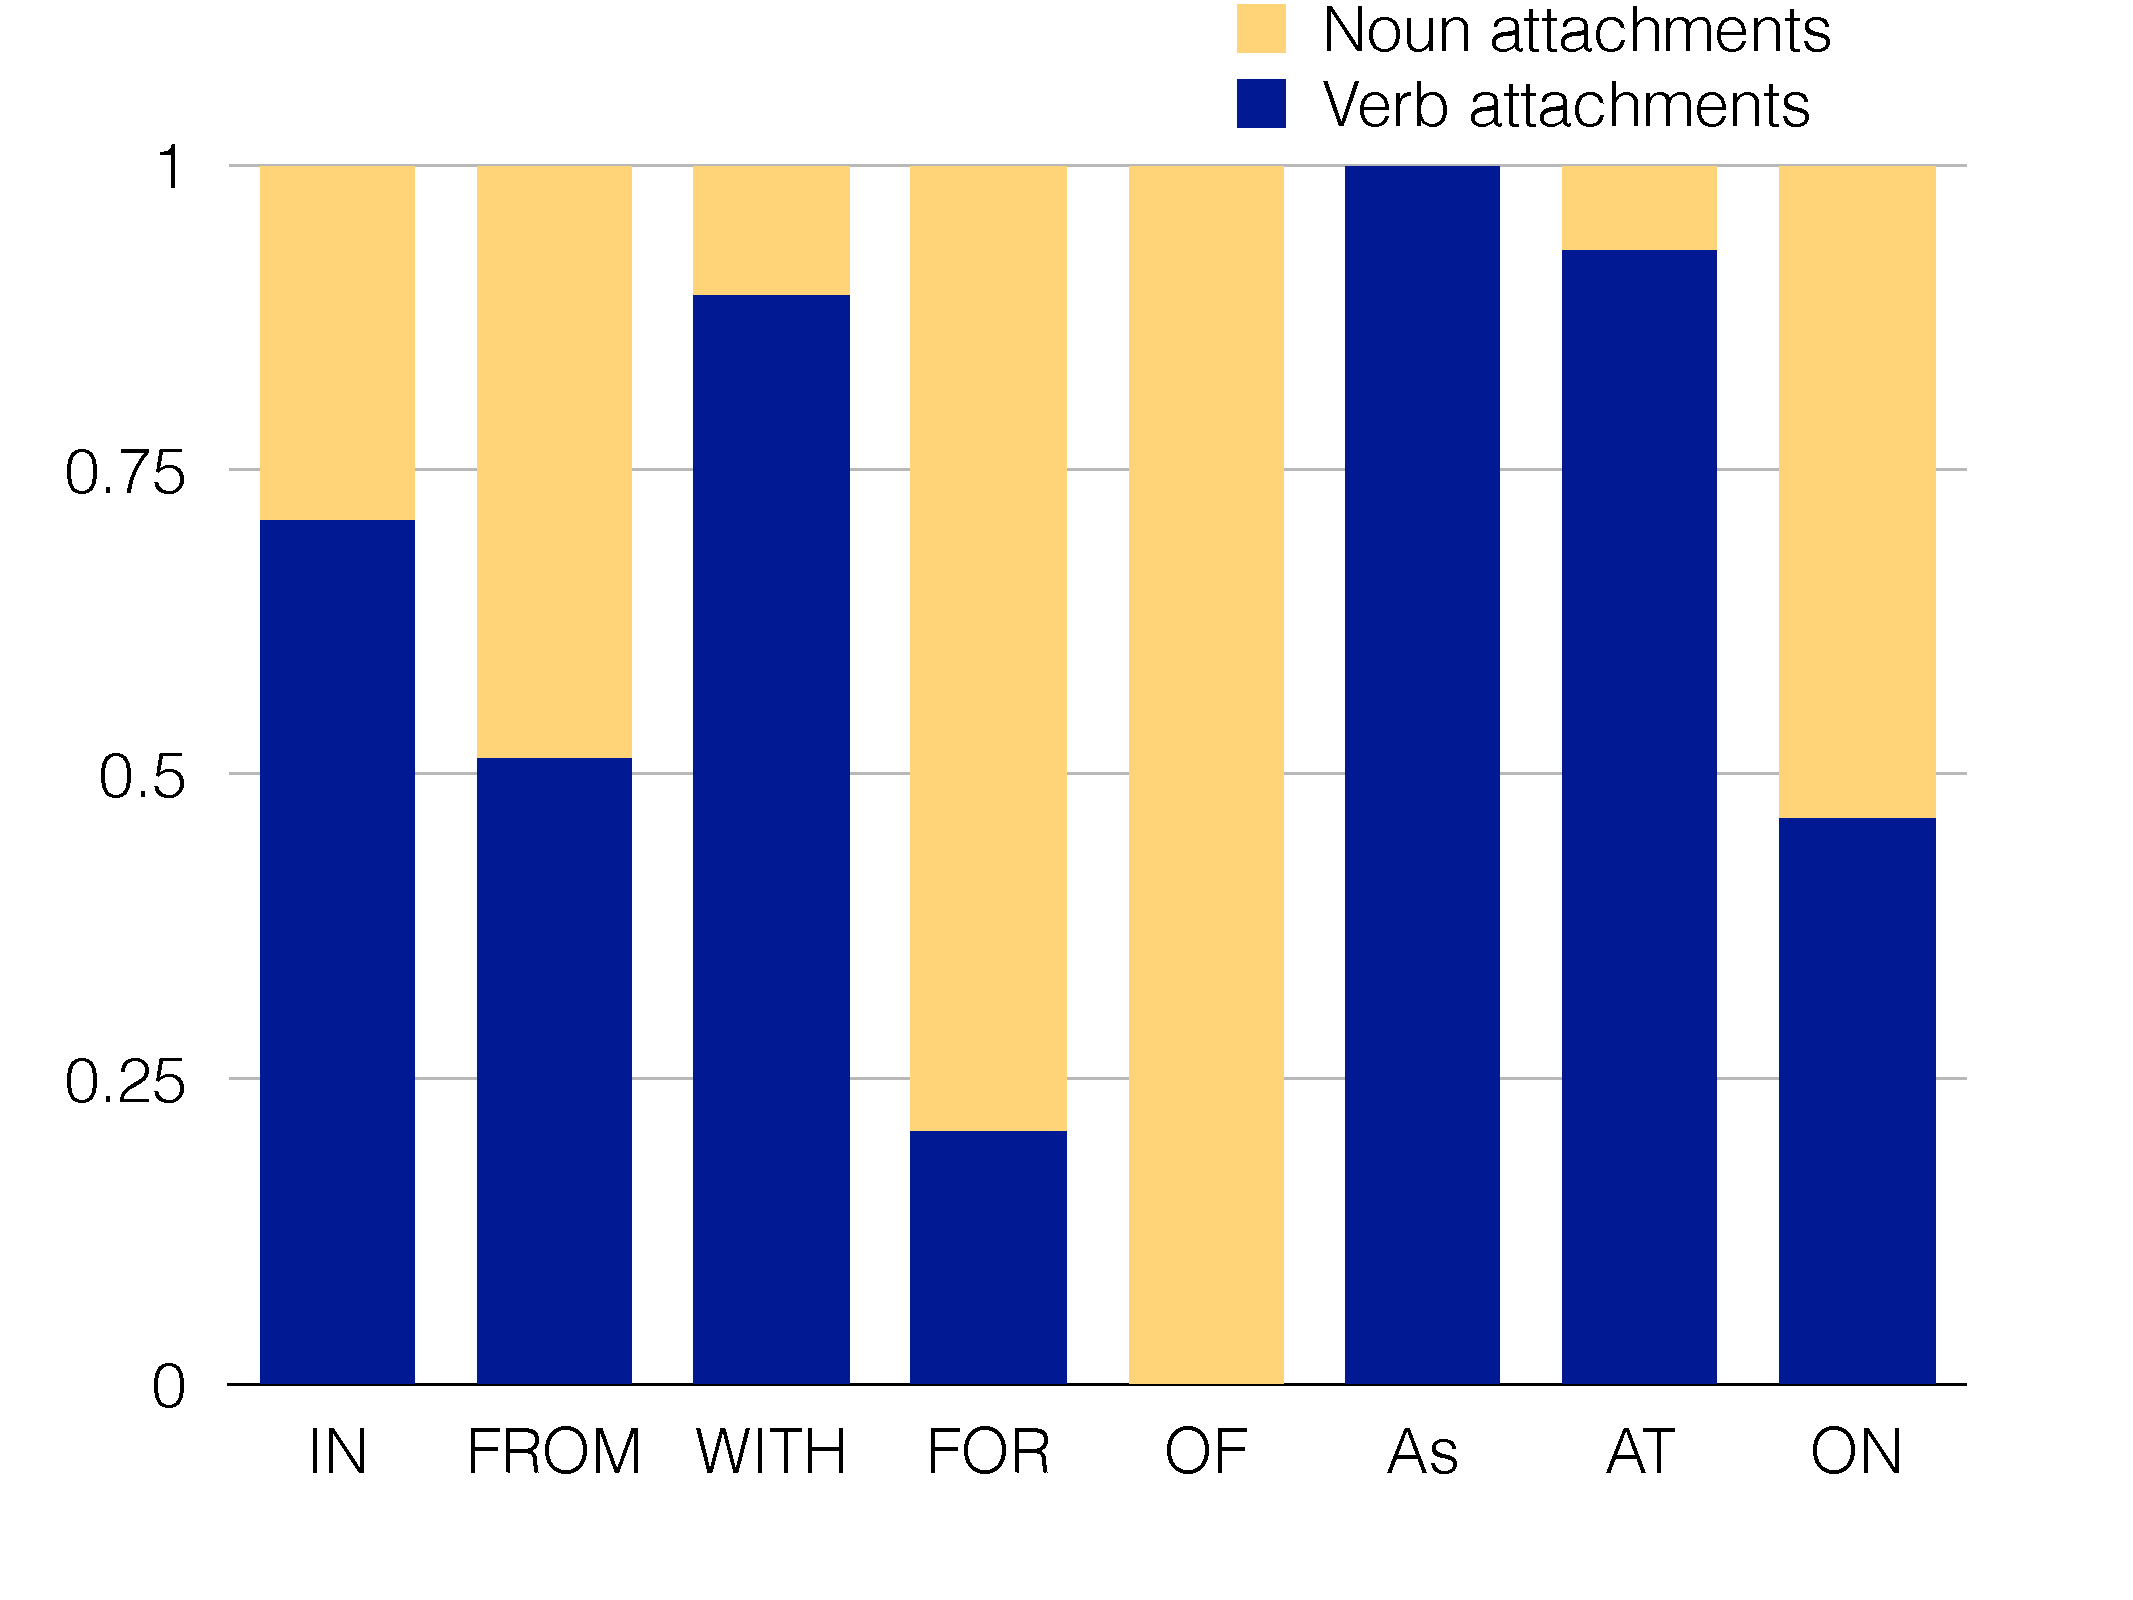
\includegraphics[width=0.85\columnwidth] {mainresults-5.pdf}
 \vspace*{-0.5cm}
 \caption{Noun vs. verb attachment proportions for frequent prepositions in the labeled NYTC dataset.}
 % The only difference in the parse trees are the PP attachment sites, resulting in trees of different structures.}
 % and hence the sentence structures are different. } 
 %
 \label{fig:distribution}
 %
 \end{figure}  

 To quantitatively assess existing tools, we analyzed performance of the widely used  Stanford parser\footnote {http://nlp.stanford.edu:8080/parser/} as of 2014,  and the established  baseline algorithm \cite{Collins95}, which has stood the test of time.
We first manually labeled PP quads from the NYTC dataset, then prepended the noun phrase appearing before the quad, effectively creating sentences made up of 5 lexical items 
$(n0\  v\  n1\  p\  n2)$.  We then applied the Stanford parser, obtaining the results summarized in Figure~\ref{fig:parser}.  The parser performs well on some prepositions, for example,  ``of", which tends to occur with noun attaching PPs as can be seen in Figure \ref{fig:distribution}.  However, for  prepositions  with an even distribution over verb and noun attachments, such as ``on", precision is as low as ~50\%. %indicating there is room for improvement.
The Collins baseline achieves 84\% accuracy on the benchmark Wall Street Journal PP dataset.  
 However, drawing a distinction in the precision of  different prepositions provides useful insights on its performance.  We re-implemented this baseline  and found that when we remove the trivial preposition,  ``of",  whose PPs are by default attached to the noun by this baseline, precision drops to 78\%. 
 This  analysis  suggests there is substantial room for improvement.
 % \highlight{For higher resolving prepositions.}


\subsection{Related Work}
\paragraph{Statistics-based Methods}
%common types of PP attachment methods in literature. 
Prominent  prior methods learn to perform PP attachment based on corpus co-occurrence statistics,  gathered either from  manually annotated training data \cite{Collins95,BrillR94} or from  automatically acquired  training data that may be noisy \cite{Ratnaparkhi98,PantelL00}.  These models collect statistics on how often a given quadruple, $\{v,n1,p,n2\}$, occurs in the training data as a verb attachment as opposed to a noun attachment.  The issue with this approach is sparsity, that is, many quadruples occuring in the test data might not have been seen in the training data.
Smoothing techniques are often employed to overcome sparsity.  For example, \cite{Collins95} proposed a back-off model that uses  subsets of the words in the quadruple, by also keeping  frequency counts of triples, pairs and single words. 
% when the test quadruple itself was not seen in the training data. 
Another approach to overcoming sparsity has been to use WordNet \cite{fellbaum98wordnet} classes, by replacing nouns with their WordNet classes \cite{Stetina97,ToutanovaMN04} to obtain less sparse corpus statistics.  Corpus-derived clusters of similar  nouns and verbs have also been used  \cite{PantelL00}.

Hindle and Rooth  proposed a lexical association approach based on how words are associated with each other \cite{HindleR93}. Lexical preference is used by  computing co-occurrence
frequencies (lexical associations) of verbs and nouns,  with prepositions. In this manner, they would discover that, for example,  the verb ``send" is highly associated with the preposition \textit{from},  indicating that in this case, the PP  is likely to be a verb attachment. 


\paragraph{Structure-based Methods}
These methods are based on  high-level  observations that are then generalized into heuristics for 
 PP attachment decisions. \cite{Kimball73}  proposed a right association method, whose premise is that a word tends to attach to another word immediately to its right.
\cite{Frazier78} introduced a minimal attachment method, which posits that  words attach to an existing non-terminal word using the fewest additional syntactic nodes. 
While simple, in practice these methods have been found to perform poorly \cite{WhittemoreFB90}.

\paragraph{Rule-based Methods}
%Different from frequency counting,
\cite{BrillR94}  proposed methods that
 learn  a set of transformation rules from a corpus. 
 %The  rules are then applied to a given PP attachment instance.
 %  and therefore, unlike the statistical methods, it is
%not necessary to store   tables  word dependencies or co-occurrence probabilities.
The rules can be too  specific to have broad applicability, resulting in low recall. 
To address low recall, knowledge about nouns, as found in  WordNet,   is used to replace certain
words in rules with  their WordNet classes. 
%This allows rules to match more  PP attachment instances


\paragraph{Parser Correction Methods}
The  quadruples formulation of the PP problem  can be seen as a simplified setting. This is because, with quadruples,  there is no need to deal with complex sentences but only well-defined quadruples of the form $\{v,n1,p,n2\}$. Thus in the quadruples setting, there are only two possible attachment sites for the PP, the $v$ and $n1$.  An alternative setting is to  work in the context of full sentences. In this setting the problem is cast as a dependency parser correction problem \cite{AttererS07,Agirre08,AnguianoC11}. That is, given a dependency parse of a sentence, with potentially incorrect PP attachments, rectify it such that the prepositional phrases attach to the correct sites. Unlike our approach, these methods do not take semantic knowledge into account.

\paragraph{Sense Disambiguation}
In addition to prior work on prepositional phrase attachment, a highly related problem is preposition sense disambiguation \cite{Hovy2011,SrikumarR13}.  Even a
syntactically correctly attached PP can  still  be semantically ambiguous with respect to questions of machine reading such as \textit{where, when,} and \textit{why}. 
Therefore, when extracting information from prepositions, the problem of preposition sense disambiguation (semantics) has to be addressed in addition to prepositional phrase attachment disambiguation (syntax). In this paper, our focus is on the latter. 
